\section{Experimental Results}
\label{experimental_results}

The presented method is evaluated in simulation and with the real hardware. After a short introduction to the experimental setup, three simulation scenarios and one real-world scenario are introduced. We compare the presented method with a sequenced MPC formulation in which arm motion and locomotion are sequenced and a conventional MPC formulation in which inequalities are formulated for individual obstacles. Scenarios are considered infeasible when following the trajectory without global replanning is not possible without violating the collision constraints.
%
\subsection{Experimental Setup}%
\label{sub:experimental_setup}

\paragraph{Hardware Setup}
The mobile manipulator used to validate this approach consists of the mobile base \textit{Clearpath\textsuperscript{TM} Boxer} and the robotic manipulator \textit{Franka Emika Panda}, see ~{Fig. \ref{fig:real_robot}}. The
resulting system has 10 degrees of freedom (DoF's) for which
the dynamics are approximated using a Runge-Kutta scheme to
obtain the discrete transition function $f(\z_t, \u_t)$.
The presented robot is equipped with low level controllers that accept commanded velocities
for all joints, one LiDAR sensor  and one
depth camera pointing forward. Laser data and camera depth images are fused into one
pointcloud using the octomap framework \cite{Hornung2013}. Polyhedrons to describe the
convex space around the links are computed using the \textit{DecompUtil} presented in
\cite{Liu2017}, into which the pointcloud generated from the vertex centers of the
occupied cells of the octomap are fed.
Joint positions for the arm are known at every time step using the encoders and the pose
of the base is estimated using SLAM.
The implementation is realized in the \textit{Robotics Operating System} (ROS) framework, as it
allows simple integration of the different components. The underlying MPC
problem is solved using \textit{FORCES-Pro} solver \cite{forcespro} and employing an interior-point method\cite{FORCESNLP}. We used a laptop with an Intel Core i7 and 32GB of RAM to run the simulations and an Intel NUC with an Intel Core i7 and 8GB to run the real-world experiments.

\paragraph{Parameter Details}%
\label{par:parameter_details}
%
The presented robot has nine links which are represented by four spheres for collision avoidance. The positions of the spheres on the kinematic chain are explicitly given in Table
\ref{tab:spheres}. Note that the robot is not fully contained in the union of spheres. For
$d_{\textrm{safety}} = 0$, this could potentially result in collision. However, much
larger spheres would result in the inability to move close to obstacles when manipulation
is requested. The parametrization with $d_{\textrm{safety}}$ allows to flexibly change
between different motion types, e.g. manipulation (low safety margin) and navigation
(large safety margin). The centers of the given spheres are also used as seed points
for the convex region
generation. Two different step size were used over the time horizon, $\Delta t_1, \Delta t_2$. All remaining parameter settings are summarized in Table
\ref{tab:parameters}. 
%
\begin{table}[!t]
  \centering
  \caption{Positions of spheres for the volumetric representation.}
  \label{tab:spheres}
  \begin{tabular}{|c|c|c|}
    \hline
    Parent Link & Offset & Radius \\
    \hline
    base link & [0, 0, 0.25] & 0.25 \\
    \hline
    base link & [0.3, 0, 0.25] & 0.25 \\
    \hline
    link 2 & [0, -0.1896, 0] & 0.2275 \\
    \hline
    link 7 & [0, 0, 0] & 0.3 \\
    \hline
  \end{tabular}
\end{table}
%
\begin{table}[h]
  \centering
  \caption{Parameter Settings}
  \label{tab:parameters}
  \begin{tabular}{|c|c|c|}
  \hline
  Parameter & Static Scenarios & Dynamic Scenario\\
  \hline
  Prediction Horizon & $11$ sec & $11s$ sec\\
  \hline
  $\Delta t_1$/$\Delta t_2$ & $0.2$/$1.0$ sec & $0.2$/$1.0$ sec\\
  \hline
  \#Planes/Link & $15$ & $15$ \\
  \hline
  $d_{\textrm{safety}}$ & $0.15$ m & $0.25$ m \\
  \hline
  $W_{\vec{e}}$ & $5.0\mat{I}_2$ & $5.0\mat{I}_2$\\
  \hline
  $w_{\theta}$ & $2.0$ & $2.0$\\
  \hline
  $W_\vq$ & $0.7 \mat{I}_7$ & $0.7 \mat{I}_7$ \\
  \hline
  $W_\vu$ & $\begin{bmatrix} 0.05\mat{I}_2 & 0 \\ 0 & 5\mat{I}_7 \end{bmatrix}$ &
  $\begin{bmatrix} 0.05\mat{I}_2 & 0 \\ 0 & 5\mat{I}_7 \end{bmatrix}$ \\
  \hline
  $w_{\textrm{slack}}$ & $10^{5}$ & $10^{5}$\\
  \hline
  \end{tabular}
\end{table}
%
%
\subsection{Manipulation Scenarios}%
\label{sub:environment_setup}

We compare our proposed method against two baseline methods: a decoupled MPC baseline (i.e., locomotion and arm motion are performed sequentially) and a coupled MPC formulation based on sphere-sphere inequality constraints, as proposed in \cite{Avanzini2018}. Moreover, as this work presents a method for local trajectory optimization, the effect of global replanning during the execution is not considered. To access our method's performance, we present simulation results for:
\begin{itemize}
    \item Static collision avoidance with a horizontal bar \cite{Avanzini2018} (Sub-section \ref{par:horizantal_bar});
    \item 2D trajectory tracking while avoiding collisions with randomly placed static obstacles (Sub-section \ref{par:randomized_obstacles});
    \item Dynamic collision avoidance with a moving obstacle (Sub-section \ref{par:dynamic_obstacle}).
\end{itemize} 
Finally, we present experimental results on a mobile manipulator performing a real manipulation task (Sub-section \ref{par:real_world}).

\paragraph{Horizontal Bar}
\label{par:horizantal_bar}
%
A horizontal bar is placed between the start and goal configuration. In contrast to the work in \cite{Avanzini2018}, no object detection is required in our approach, as the sensed point cloud is fed directly into the convex region generator. The base's global path consists of a simple straight-line motion to a pose behind the bar. The motion of the manipulator and the generated convex regions for the last link of the kinematic chain are depicted in ~{Fig. \ref{fig:bar_motion}}. 
% Improved flexibility
The advantage of whole-body optimization can be extracted when the horizontal bar is placed at a lower $z$-positions. In ~{Fig. \ref{fig:feasibility_issue}}, such a situation is visualized for $z=1.3$. In the visualized case, it is not possible to move underneath the bar with the sequenced approach. On the other hand, the coupled method can navigate safely avoiding collision by moving the arm into an extended position in which the absolute height is smaller than when having it folded.
%
\begin{figure}[h]
    \centering
    \begin{subfigure}[b]{0.45\linewidth}
        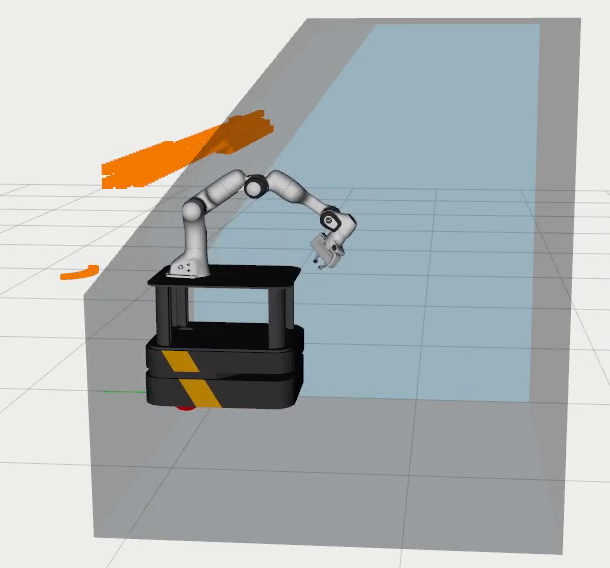
\includegraphics[width=0.9\textwidth]{bar/adv_coupling.png}
        \caption{coupled}
    \end{subfigure}
    \begin{subfigure}[b]{0.425\linewidth}
        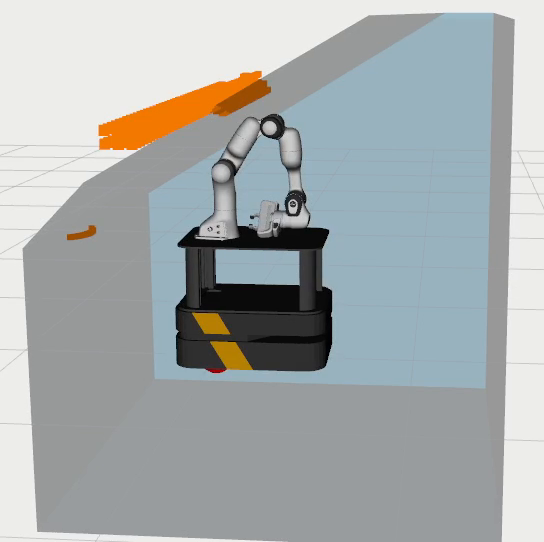
\includegraphics[width=0.9\textwidth]{bar/adv_decoupling.png}
        \caption{decoupled}
    \end{subfigure}
    \caption{Advantage of coupled MPC when moving underneath a horizontal bar (orange). }
    \label{fig:feasibility_issue}
\end{figure}
%
\begin{figure}[h]
  \centering
  \begin{subfigure}[b]{0.32\linewidth}
    \includegraphics[width=1.0\textwidth]{bar/sequence_pic1.png}
    \caption{$t=0sec$}
  \end{subfigure}
  \begin{subfigure}[b]{0.32\linewidth}
    \includegraphics[width=1.0\textwidth]{bar/sequence_pic2.png}
    \caption{$t=6sec$}
  \end{subfigure}
  \begin{subfigure}[b]{0.32\linewidth}
    \includegraphics[width=1.0\textwidth]{bar/sequence_pic3.png}
    \caption{$t=17sec$}
  \end{subfigure}
  \begin{subfigure}[b]{0.32\linewidth}
    \includegraphics[width=1.0\textwidth]{bar/sequence_pic4.png}
    \caption{$t=25sec$}
  \end{subfigure}
  \begin{subfigure}[b]{0.32\linewidth}
    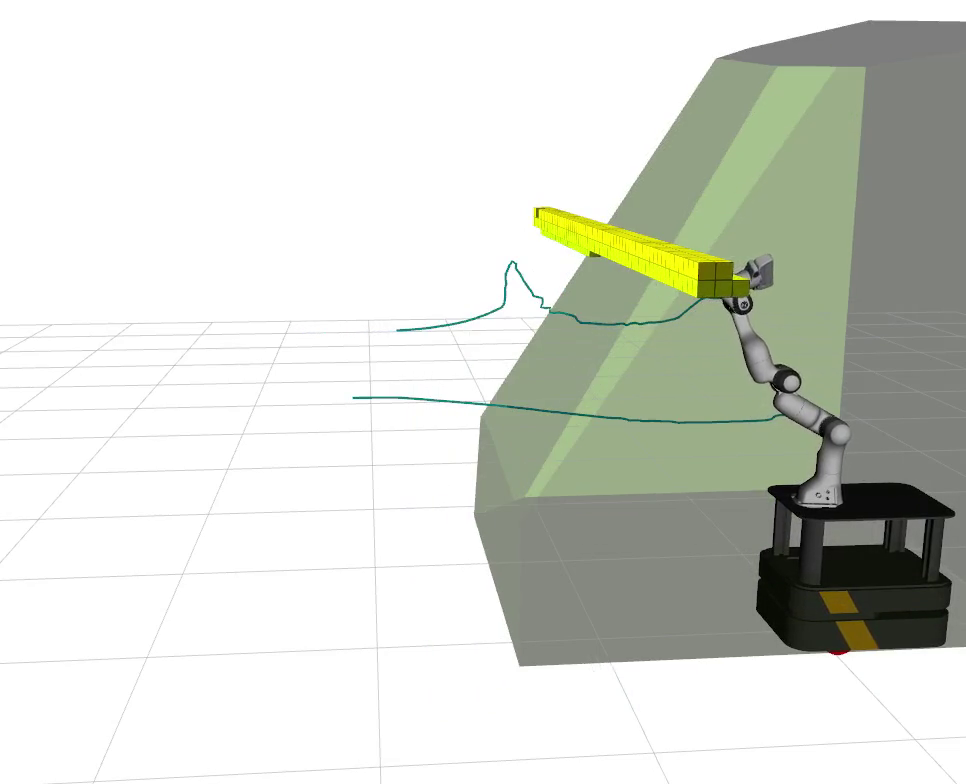
\includegraphics[width=1.0\textwidth]{bar/sequence_pic5.png}
    \caption{$t=32sec$}
  \end{subfigure}
  \begin{subfigure}[b]{0.32\linewidth}
    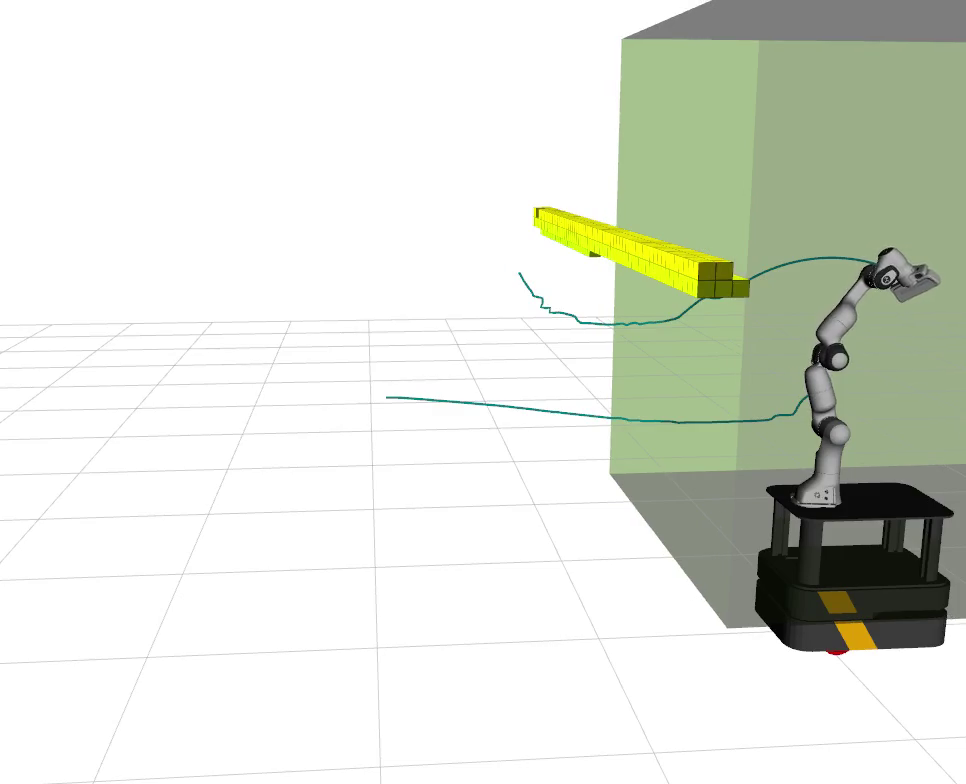
\includegraphics[width=1.0\textwidth]{bar/sequence_pic6.png}
    \caption{$t=42sec$}
  \end{subfigure}
  \caption{Avoiding an horizontal bar. The convex region
for the last link of the kinematic chain.}%
  \label{fig:bar_motion}
\end{figure}

%
\paragraph{Randomized Obstacles}%
\label{par:randomized_obstacles}
%
In this scenario, the robot is placed in an unstructured environment with several static obstacles. A global path for the base to reach the goal is computed, but the path is blocked with randomly
generated obstacles, uniformly distributed on the intervals $x \in [2m, 5m], y \in [-2m, 2m], z
\in [0m, 2m]$. Only those obstacles visible to the LiDAR sensors are available for the global planner which generates a path in the 2D plane for the base's motion. Among the randomly generated cases, only those that are feasible for an MPC trajectory optimizer are considered. Two examples for infeasible cases are depicted in ~{Fig. \ref{fig:infeasible}}.

\begin{figure}[!t]
    \centering
    \begin{subfigure}[b]{0.48\linewidth}
        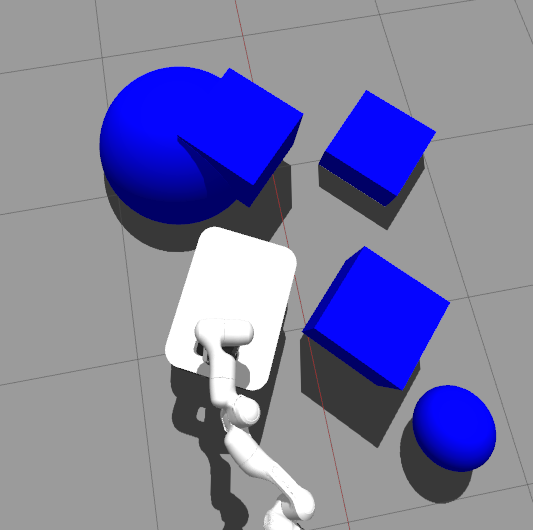
\includegraphics[height=0.9\linewidth]{randObst/infeasible1.png}
    \end{subfigure}
    \begin{subfigure}[b]{0.48\linewidth}
        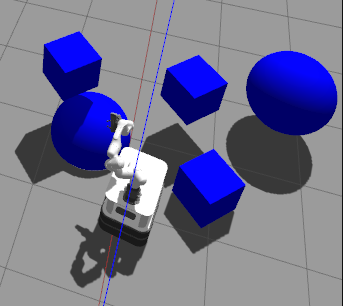
\includegraphics[height=0.9\linewidth]{randObst/infeasible2.png}
    \end{subfigure}
    \caption{Example for infeasible cases, that were excluded from the test set in randomized scenario.}
    \label{fig:infeasible}
\end{figure}
%
\begin{figure}[t]
  \centering
  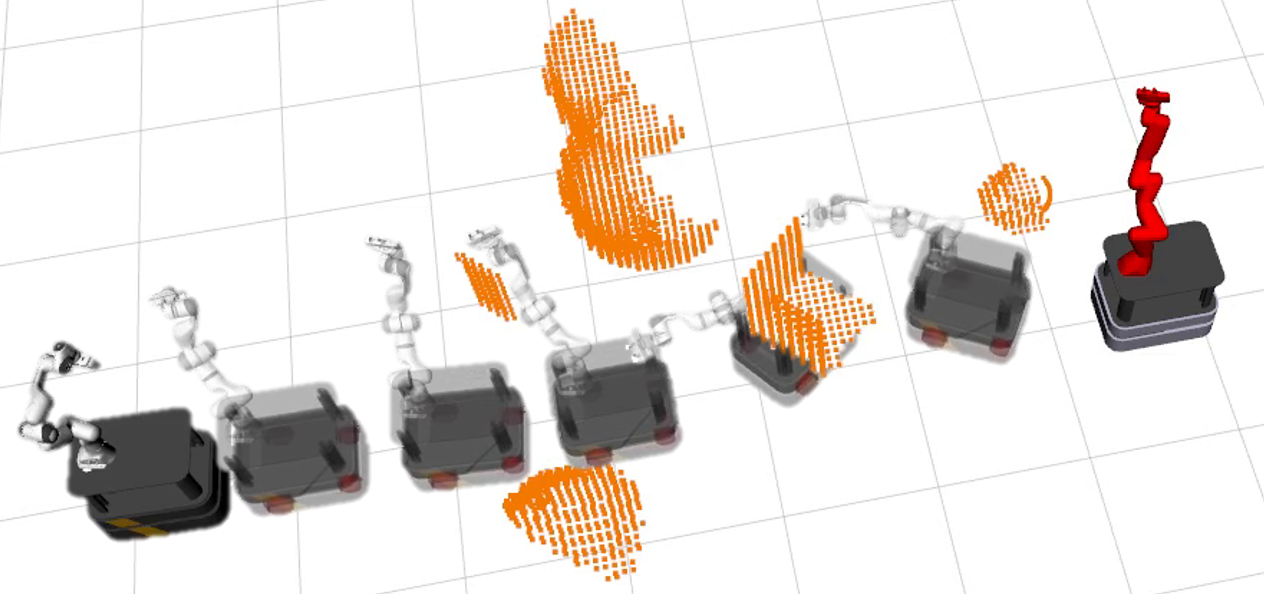
\includegraphics[width=0.8\linewidth]{randObst/trajectory.png}
  \caption{Five obstacles avoidance, final configuration in red, occupied voxels in the octomap are represented in orange.}%
  \label{fig:case_2_example}
\end{figure}
%
\begin{figure}[h]
  \centering
  \begin{subfigure}[b]{0.45\linewidth}
    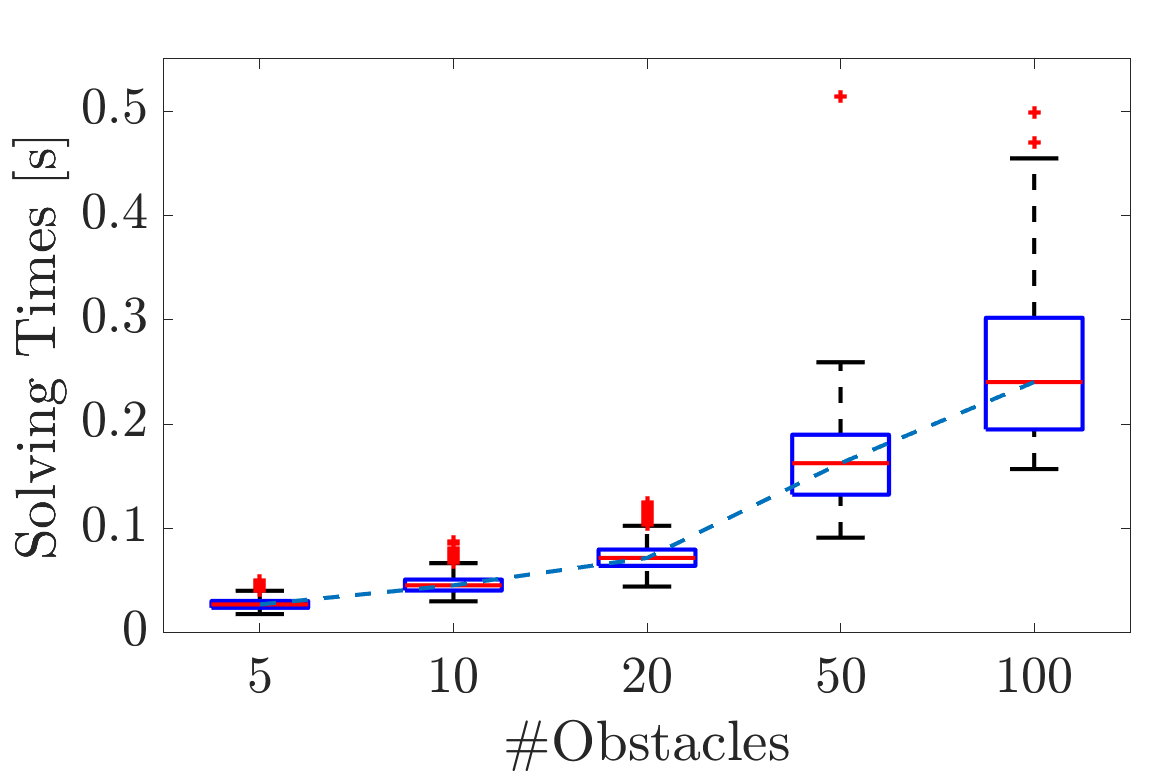
\includegraphics[height=0.7\linewidth]{randObst/increase_solverTimes_spheres.png}
    \caption{Obstacles as spheres}
  \end{subfigure}
  \begin{subfigure}[b]{0.45\linewidth}
    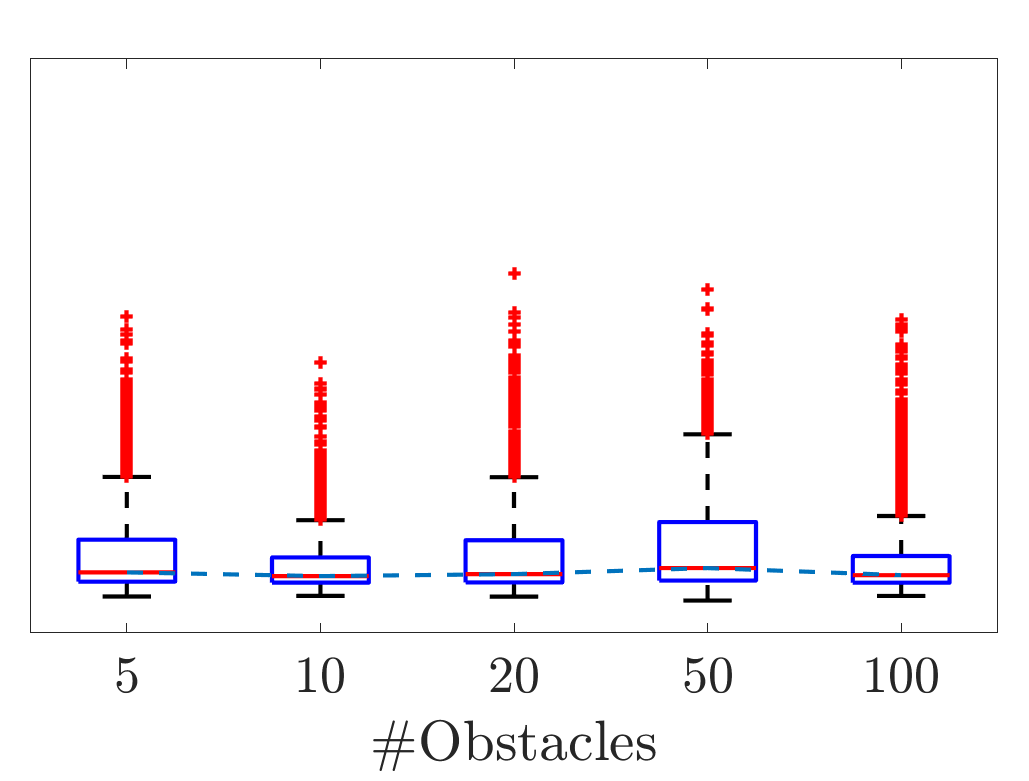
\includegraphics[height=0.7\linewidth]{randObst/increase_solverTimes_convex.png}
    \caption{Convex regions}
  \end{subfigure}
  \caption{Comparison solver performance for an increasing number of obstacles.}%
  \label{fig:randObst_solver}
\end{figure}
\begin{table}
    \centering
    \begin{tabular}{|c|c|c|}
        \hline
         & decoupled & coupled \\
         \hline
         mean & 219.65s & 113.822s \\
         std. deviation & 24.21s & 8.35s\\
         min & 199.27s & 106.83s \\
         max & 270.25s & 131.24s \\
         \hline
    \end{tabular}
    \caption{Compared execution times coupled and decoupled approach for cases that were feasible for both methods.}
    \label{tab:randObst}
\end{table}
%

A successful trajectory of the coupled MPC planner is depicted in ~{Fig. \ref{fig:case_2_example}}. A key advantage of our method is that when the environment is densely populated with obstacles, the solving times are not affected when using convex regions to represent the free space, see Fig. \ref{fig:randObst_solver}. Explicitly formulating sphere-sphere inequality constraints results in an increase of solving time as the environment becomes more densely populated with obstacles. Note that convex region generation becomes only beneficial as the number of obstacles exceeds a critical value, in this case, for 50 obstacles.
Furthermore, parallelizing the locomotion and arm motion allows to reduce the mean overall operational time by 48\%, see ~{Table \ref{tab:randObst}}.
%

\paragraph{Dynamic Obstacle}%
\label{par:dynamic_obstacle}

Here, we evaluate dynamic collision avoidance with a single moving obstacle for different obstacle's velocities. As dynamic object detection and velocity estimation are out of the scope of this work, the state of the obstacle is assumed to be known to the robot during the entire process. In Fig. \ref{fig:dynamic_case}, the experiment is visualized. The goal pose (light grey) is to be reached but a moving sphere, conflicting the goal, must be avoided at all time. 
The proposed MPC formulation's reactivity is investigated using the clearing distance $d_{\textrm{clear}} = \min_i{\norm{\vp^{\textrm{dyn}} - \vp_{i}} - r_i - r_d^{\textrm{dyn}}}$ and the distance to target, $d_{\textrm{target}} = \norm{\vec{z}_{\textrm{des}} - \vec{z}}$, where $\vec{z}_{\textrm{des}}$ is composed of the desired base and arm configuration. Different velocities ($\vec{v}_d^{\textrm{dyn}}$) and different heights ($z_{\textrm{obs}}$) of the moving obstacles were investigated. Fig. \ref{fig:dynamic_distances} shows that our approach successfully avoids collision with dynamic obstacles when moving towards the goal. 
%
\begin{figure}[h]
  \centering
%  \includegraphics[width=1.0\linewidth]{dynFig.png}
  \begin{subfigure}[b]{0.4\linewidth}
    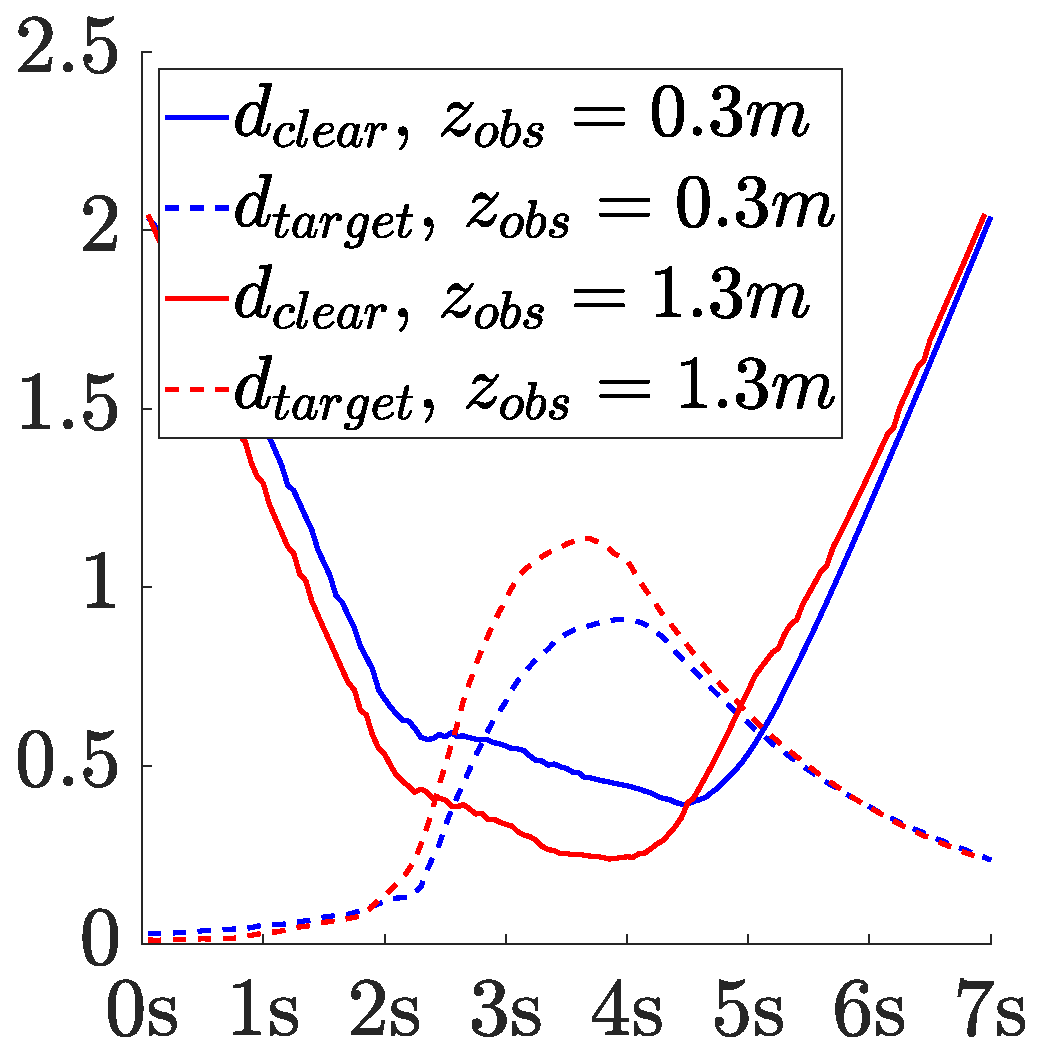
\includegraphics[width=1.0\textwidth]{dynamic/distances_slow}
        \caption{$\norm{\vec{v}_d} = 0.2m/s$}
  \end{subfigure}
  \begin{subfigure}[b]{0.4\linewidth}
    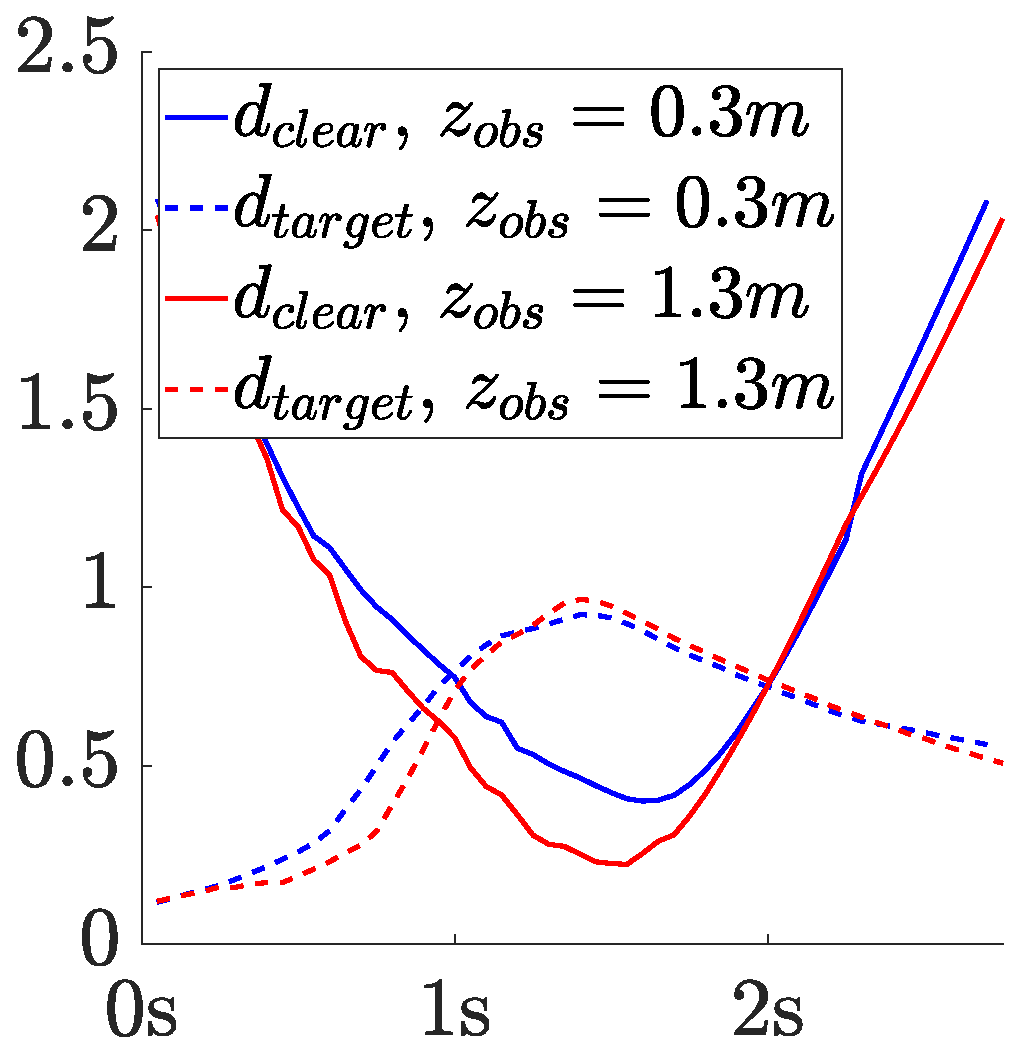
\includegraphics[width=1.0\textwidth]{dynamic/distances_fast}
    \caption{$\norm{\vec{v}_d} = 0.5m/s$}
  \end{subfigure}
  \caption{Clearance from moving obstacle and distance to target position for different obstacle velocities.}%
  \label{fig:dynamic_distances}
\end{figure}
%
\begin{figure}[h]
  \centering
  \begin{subfigure}[b]{0.23\linewidth}
    \includegraphics[width=1.0\textwidth]{dynamic/sequence_pic1.png}
    \caption{$t=0sec$}
  \end{subfigure}
  \begin{subfigure}[b]{0.23\linewidth}
    \includegraphics[width=1.0\textwidth]{dynamic/sequence_pic2.png}
    \caption{$t=1sec$}
  \end{subfigure}
  \begin{subfigure}[b]{0.23\linewidth}
    \includegraphics[width=1.0\textwidth]{dynamic/sequence_pic3.png}
    \caption{$t=2sec$}
  \end{subfigure}
  \begin{subfigure}[b]{0.23\linewidth}
    \includegraphics[width=1.0\textwidth]{dynamic/sequence_pic4.png}
    \caption{$t=3sec$}
  \end{subfigure}
  \caption{Motion avoiding moving obstacle (red) while attempting to reach target (light grey).}%
  \label{fig:dynamic_case}
\end{figure}
%
\paragraph{Real-World Experiment}
\label{par:real_world}
%
\begin{figure}[ht]
  \centering
  \begin{subfigure}[b]{0.23\linewidth}
    \includegraphics[width=1.0\textwidth]{real/sequence_pic1.png}
  \end{subfigure}
  \begin{subfigure}[b]{0.23\linewidth}
    \includegraphics[width=1.0\textwidth]{real/sequence_pic2.png}
  \end{subfigure}
  \begin{subfigure}[b]{0.23\linewidth}
    \includegraphics[width=1.0\textwidth]{real/sequence_pic3.png}
  \end{subfigure}
  \begin{subfigure}[b]{0.23\linewidth}
    \includegraphics[width=1.0\textwidth]{real/sequence_pic4.png}
  \end{subfigure}
  \caption{Trajectory in mock-up store avoiding obstacles, goal configuration in light grey.}%
  \label{fig:real_case}
\end{figure}
%
We evaluated the presented method in real-world scenarios in a simple pick \& place setup. ~{Fig. \ref{fig:real_robot}} depicts the experimental scenario, where the robot picks up an object on the left (pose in light green) and moves to the target pose (pose in light red) without colliding with the obstacle visualized in light blue. Intermediate poses of the successful trajectory are visualized in Fig. \ref{fig:real_case}. A video of the experiment is attached to this work.
%
